\documentclass{jdrp}

\bibliography{tex/references} 

\newcommand*{\crg}{{\aurebesh\Large \$}} % Symbol for Galactic Credits

\hypersetup{  
  pdfinfo={  
    Title={SWR - La Citadelle Hurlante},
    Subject={Scénario, Citadelle Hurlante},
    Author={Marthym},
    Keywords={starwars,savage,worlds,jdr,scenario},  
    Copyright={Do What The Fuck You Want To Public License}
  }  
} 

\begin{document}

	\begin{titlepage}

	\begin{center}
		\hspace*{\vfill}
		\noindent\Huge\jedifont{Star Wars Redemption}\\ 
		\noindent\fontsize{50}{70}\jedifont{\$}
		\noindent\fontsize{50}{70}\jedifont{\#}\\
		\noindent\fontsize{50}{60}\jedifont{La Citadelle Hurlante}
		\hspace*{\vfill}
	\end{center}

	%\hspace*{\vfill}

	\noindent\makebox[\textwidth]{
		\includegraphics[width=\paperwidth]{swr-class/_img/cover-bg.png}}
	\begin{tikzpicture}[overlay]
		\node[minimum width=200pt,minimum height=200pt, rotate=0] at (2,5){\includegraphics[width=200pt]{_img/places/citadel-of-ktath-atn.png}};
	\end{tikzpicture}}
	\end{titlepage}

	\onecolumn
	\section{avant propos}
	
	\begin{wrapfigure}{R}{180pt}
		\centering
		\includegraphics[width=180pt]{_img/pnjs/aphra.png}
		\caption{\label{fig:aphra}Docteur Aphra}
		\vspace{1\baselineskip}
		\includegraphics[width=180pt]{_img/pnjs/ktath-atn-queen.png}
		\caption{\label{fig:ktath-atn-queen}Reine de Ktath’Atn}
	\end{wrapfigure}

	Ce scénario est pleinement inspiré du spin-off entre la série \citetitle{starwars-marvel} & \citetitle{starwars-aphra}. Il est initialement prévue pour être joué selon les règles des \citetitle{jdrp-starwars}. Le scénario est écrit pour une petite équipe de héros (3 à 5) déjà formé mais la première scène peu être facilement adapté. Un padawan ou un Jedi est nécessaire, si votre équipe n’en contient pas, il faudra soit adapter le scénario pour l’un de vos joueurs, soit ajouter un PNJ padawan.

    \bigbreak
    
    Le scénario se passe peu après la destruction de la première Etoile de la mort par le jeune Luke Skywalker. Vos héros se trouvent embarqués par le Doctor Aphra, archéologue un peu frappée à la morale douteuse. Cette dernière a besoin d’une forme de vie organique "intéressante" à présenter à la reine de la Citadelle Hurlante pour accéder à la mémoire d’un ancien Jedi. Aucun padawan ne peu refuser une offre pareille...

    \bigbreak

    Ce scénario est initialement pensé pour des héros tendant vers le coté lumineux de la Force mais je proposerais chaque fois que nécessaire une version pour le coté obscur.

    \vspace*{\fill}

	\subsection{Licence}
	\noindent DO WHAT THE FUCK YOU WANT TO PUBLIC LICENSE\\
    Version 2, December 2004
    \vspace{-2.5\baselineskip}
	\begin{flushright}
		\includegraphics[width=70pt]{swr-class/_img/wtfpl-badge.png}
	\end{flushright}

	\twocolumn

	\section{Docteur Aphra}

\subsection{introduction}
Ce scénario commence dans une cantina pas vraiment accueillante d’Horox III. Les héros aspirent à un peu de repos bien mérité après une mission pour l’alliance qui n’a pas vraiment été un franc succès.

\lettrine{\jedifont{\$}} Ils avaient pour objectif d’identifier l’origine d’un trafic de matrices droïde modifiées pour le combat. Malheureusement après deux semaines de recherches et d’interrogatoires infructueux, tout ce qu’ils ont réussi à faire, c’est se prendre une correction par l’un des fameux droïdes modifiés et perdre la trace de leur trafiquant quelque part sur \textbf{Horox III}.

\lettrine{\jedifont{\#}} Les héros étaient en mission pour l’empire. Ils sont à la recherche d’un individu capable de modifier les matrices de droïde pour en faire des droïdes de combat plutôt performant. Le seigneur Vador se montre très intéressé car il souhaite se monter une armée personnelle.

\begin{paperbox}{Objectif}
Les héros sont à la recherche d’un trafiquant de matrices de droïdes.
\end{paperbox}

\subsection{Viens voir le docteur}
\noindent\includegraphics[width=\linewidth]{_img/places/cantina-horox-iii.jpg}
Les voilà donc ruminant leur échec dans un bar quand entre une femme, brune, mince, un bonnet et des lunettes d’aviateur sur la tête. L’horoxien au bar lève la tête et semble, l’espace d’un instant, surpris. Puis il se reprend et interpelle violemment la femme :

\begin{quotebox}
- \textbf{barman} Aphra ! Tu ne manques pas d’aplomb de te repointer ici ! Les droïdes que tu m’a refilés, c’était de la merde. Ils ont pas tenu 10 minutes !\\
- \textbf{Aphra} En face de ta sale gueule ça m’étonne pas !\\
- \textbf{barman} Attrapez là, on va lui faire sa fête !
\end{quotebox}

Les \nameref{sec:horoxian-barfly}, jusqu’alors calmes, occupés à leurs consommations se lèvent et commencent à pousser les tables. L’ambiance devient très tendue, la bagarre est inévitable.

Si vos joueurs ont un peu de jugeote, ils comprennent qu’\nameref{sec:aphra} a quelque chose à voir avec les matrices modifiées qu’ils recherchent, ou qu’au moins elle peut les aider. S’ils ne comprennent pas incitez les à entrer dans la danse avec une bouteille perdue par exemple.

\begin{paperbox}{Baston de bar}
Comptez 2 \nameref{sec:horoxian-barfly} par héros pour que ça soit un peu marrant. Faites aussi en sorte qu’ils n’utilisent pas leurs armes, ça serait trop facile sinon. En gros la mission était finie et ils n’ont pas pris leurs armes avec eux, ou les armes sont interdites dans la cantina.

Au pire, s’ils s’en sortent pas, les \nameref{sec:horoxian-barfly} vont fuir.
\end{paperbox}

\subsection{Docteur \& Queen}

Une fois la baston terminée, les héros interpellent \nameref{sec:aphra}, s’ils n’en font rien, c’est elle qui les accoste.

Soit ils lui demandent des infos sur les matrices de droïdes et elle leur propose un marché, soit, elle leur demande de l’aide pour résoudre un problème en échange d’argent ou d’un artefact Jedi. Tout dépend ce qui fait rêver vos joueurs.

\nameref{sec:aphra} leur explique alors son problème. Elle possède un artefact, le cristal de Rur, contenant la mémoire d’un Jedi mais elle ignore comment l’ouvrir. Par chance, une fois par an, la \nameref{sec:ktath-atn-queen} organise une réception durant laquelle elle accorde un vœu à la personne qui lui apportera la forme de vie organique la plus “étonnante”. Et il se trouve que cette réception a justement lieu demain soir, et présenter un spécimen d’humain sensible à la Force par les temps qui courent leur assurerait à coup sûr l’accès au vœu. S’il se pose la question, l’artefact réagit aux êtres sensibles à la Force.

\bigbreak

Une fois la discussion terminée, laissez les héros récupérer leurs armes et faire le plein de munition puis en route pour \textbf{Ktath’Atn.}

\begin{paperbox}{Objectif}
Aider \nameref{sec:aphra} à ouvrir l’artefact pour obtenir les renseignements sur le trafic de matrices.
\end{paperbox}

	\section{Personnages}
Les personnages avec un ‘ \textbf{*} ’ sont des Jokers, ils possèdent une fiche de perso jouable. 

\subsection{Reine de Ktath’Atn*} \label{sec:ktath-atn-queen}
\begin{figure}[h!]
    \centering
    \includegraphics[height=250pt]{_img/pnjs/ktath-atn-queen.png}
\end{figure}
\subsubsection{Background}
Femme mystérieuse qui dirige la \textbf{Citadelle Hurlante} sur la planète Ktath’atn en l’an 0. Chaque année, elle organise une soirée durant laquelle elle reçoit de nombreux civils venus lui présenter des formes de vie organiques “intéressantes”. Celui qui présente la forme de vie la plus intéressante se voit alors accorder un vœu par la reine.
\newpage
\begin{paperbox}{Pouvoirs de la reine}
La reine, grâce à sa compétence \textit{Symbiose Parfaite} possède des pouvoirs non basés sur la Force. Ces pouvoirs font d’elle un combattant redoutable malgré son illusoire absence d’aptitudes au combat. Voici le fonctionnement et les effets de ces pouvoirs, jouez-le comme l’Arcane \textit{Science \'Etrange} de \citetitle{savage-worlds} mais sans l’objet associé.
\bigbreak
\begin{rebelist}
    \item \textbf{Téléportation [3pt]}: Grâce à sa faculté de téléportation, la reine est capable de se déplacer instantanément d’un endroit à l’autre de la citadelle. Ce pouvoir compte pour le déplacement du round. Pour se téléporter vers un endroit qu’elle ne voit pas, la reine a un malus de \textbf{-2}. En cas d’échec critique, un 1, la reine subit \textbf{2d6} de dommages.
    \item \textbf{Choc Psychique [2pt]}: La reine est capable d’émettre une sorte d’onde psychique qui va étourdir tous les ennemis sur un rayon de 6m autour d’elle. En cas de succès, les victimes doivent réussir un jet de \textbf{Vig}ueur sinon elles se retrouvent secouées. En cas de Relance, le jet de \textbf{Vig}ueur subit un malus de \textbf{-2}.
    \item \textbf{\'Eclair [1-3pt]}: La reine concentre sa psyché en une énergie tangible. Sous la forme d’un éclair qui foudroie ses ennemis. Elle peut créer 1 à 3 éclairs, chaque éclair coûte un point de pouvoir supplémentaire. S’ils touchent chaque éclair fait \textbf{2d6}. La puissance peut être montée à \textbf{3d6} si la reine concentre trois éclairs en un seul point.
    \item \textbf{Dissipation [3pt]}: La reine est capable de contrer les pouvoirs de la Force. Elle peu dissiper un pouvoir en cours ou, si elle est en attente, contrer un pouvoir dont elle est la cible, le jet de \textit{Symbiose} vient donc contrer le jet de Force.
    \item \textbf{Augmentation [2pt]}: La reine peut augmenter l’un de ses Traits d’un dé, voire deux avec une Relance. L’augmentation dure 3 tours et demande \textbf{1pt} de pouvoir supplémentaire par tour.
\end{rebelist}
\end{paperbox}
\newpage

\begin{tikzpicture}[overlay, anchor=north]
    \node at (9,2) {\includegraphics[height=0.99\paperheight]{_img/pnjs/fiche-ktath-atn-queen.pdf}};
\end{tikzpicture}

\clearpage

\subsection{Aphra} \label{sec:aphra}
\begin{figure}[h!]
    \centering
    \includegraphics[height=250pt]{_img/pnjs/aphra.png}
\end{figure}
\subsubsection{Background}
Chelli Lona Aphra, nommée d’après sa défunte mère Lona Aphra, surnommée Boop par son père, et appelée Aphra par le reste du monde, était une archéologue et contrebandière. Elle travailla notamment pour Dark Vador après la destruction de l’Étoile de la Mort. Jeune femme séduisante au tempérament bien trempé, brune avec des électrotatouages sur le bras droit, elle sait ce qu’elle veut, admire les gens de pouvoir, et ne fait confiance qu’à elle-même pour survivre.

\subsubsection{Traits}

\begin{itemtable}[ c c c c c ]
    \textbf{Agi} & \textbf{Int} & \textbf{\^Ame} & \textbf{For} & \textbf{Vig} \\
    d8           & d12          & d4             & d6           & d6           
\end{itemtable}
\begin{itemtable}[ l X ]
    \textbf{Allure}      & 6 \\
    \textbf{Compétences} & Connaissance(Archéologie) d10, \newline Réparation d10, Tir d8 \\
    \textbf{Atouts}      & Bidouilleur, Voleur, Acolyte(Wookie)
\end{itemtable}

\subsubsection{Défense}
\begin{itemtable}[ c c ]
    \textbf{Parade}     & \textbf{Résistance} \\
    6                   & 5 
\end{itemtable}

\newpage

\subsection{Bombinax} \label{sec:bombinax}
\begin{figure}[h!]
    \centering
    \includegraphics[height=250pt]{_img/pnjs/bombinax.png}
\end{figure}

\subsubsection{Background}
Bombinax est le chef de la garde de la Citadelle. Il est aussi proche de la reine et fait partie de ces lieutenants. C’est un homme brutal, totalement dévoué à la reine. Il n’a pas pour habitude de discuter les ordres de la reine, si elle lui ordonnait de s’ouvrir les veines, il le fera dans l’instant. Mais il n’est pas stupide pour autant, il est perspicace et très méfiant. Il est cependant très sensible au sarcasme, notamment concernant sa blessure au visage.

\subsubsection{Traits}

\begin{itemtable}[ c c c c c ]
    \textbf{Agi} & \textbf{Int} & \textbf{\^Ame} & \textbf{For} & \textbf{Vig} \\
    d4-2         & d6           & d4             & d10          & d10           
\end{itemtable}
\begin{itemtable}[ l X ]
    \textbf{Allure}      & 6 \\
    \textbf{Compétences} & Combat d10, Intimidation d6, \newline Lancer d8 \\
    \textbf{Handicap}    & Susceptible (-2 pour contrer Sarcasme)
\end{itemtable}

\begin{itemtable}[ l X ]
    \textbf{Arme}        & \textbf{Dégâts} \\
    Marteau énergétique  & For+2d6
\end{itemtable}

\begin{itemtable}[ c c ]
    \textbf{Parade}     & \textbf{Résistance} \\
    7                   & 7 (+6 Armure)
\end{itemtable}

\newpage
\subsection{Varroa} \label{sec:varroa}
\begin{figure}[h!]
    \centering
    \includegraphics[height=250pt]{_img/pnjs/varroa.png}
\end{figure}

\subsubsection{Background}
Conseiller principal de la reine, Varroa est son lieutenant le plus ancien. Beaucoup de secrets planent autour de cet individu, des rumeurs de rituels étranges. Varroa n’est pas un combattant mais il est manifeste qu’il pratique une sorte de magie potentiellement très dangereuse.

\subsubsection{Traits}

\begin{itemtable}[ c c c c c ]
    \textbf{Agi} & \textbf{Int} & \textbf{\^Ame} & \textbf{For} & \textbf{Vig} \\
    d2           & d10          & d10            & d2           & d2           
\end{itemtable}
\begin{itemtable}[ l X ]
    \textbf{Allure}      & 6 \\
    \textbf{Compétences} & Connaissance(Symbiote) d12, \newline Soin d6, Discrétion d6 \\
    \textbf{Atouts}      & Arcane(Symbiote), \newline Don des langues \\
    \textbf{Handicaps}   & Frêle, Loyal
\end{itemtable}
\begin{itemtable}[ c c ]
    \textbf{Parade}     & \textbf{Résistance} \\
    2 (-1 Frêle)        & 2
\end{itemtable}

\newpage
\subsection{Vespinax} \label{sec:vespinax}
\begin{figure}[h!]
    \centering
    \includegraphics[height=250pt]{_img/pnjs/vespinax.png}
\end{figure}

\subsubsection{Background}
Chef du service de renseignement de la reine, Vespinax est aveugle depuis toujours mais elle a développé ses autres sens au point qu’elle y voit mieux que le commun des mortels (et des immortels). Elle est sans pitié avec ses proies. Beaucoup moins puissante de son confrère Bombinax, Vespinax est une adversaire très agile et difficile à atteindre.

\subsubsection{Traits}

\begin{itemtable}[ c c c c c ]
    \textbf{Agi} & \textbf{Int} & \textbf{\^Ame} & \textbf{For} & \textbf{Vig} \\
    d8           & d6           & d4             & d6           & d4           
\end{itemtable}
\begin{itemtable}[ l X ]
    \textbf{Allure}      & 6 \\
    \textbf{Compétences} & Combat d12, Discrétion d10, \newline Perception d8 \\
    \textbf{Atouts}      & Frappe foudroyante, \newline Grande esquive, Contre-attaque \\
    \textbf{Handicap}    & Loyal, Rancunier, Sanguinaire
\end{itemtable}

\begin{itemtable}[ l X ]
    \textbf{Arme}        & \textbf{Dégâts} \\
    Baton ènergétique    & For+d4+d6 (\'Energie)
\end{itemtable}

\begin{itemtable}[ c c ]
    \textbf{Parade}     & \textbf{Résistance} \\
    8                   & 4 (+2 tête)
\end{itemtable}
	\section{Bestiaire}

\subsection{Pilier de bar Horoxien} \label{sec:horoxian-barfly}
\begin{figure}[h!]
    \centering
    \includegraphics[height=200pt]{_img/bestiary/horoxian-barfly.png}
\end{figure}
\paragraph{Background}
Pas très malin, le pilier de bar horoxian se cache dans les cantina d’Horox III. Passe le plus clair de son temps à picoler et a refaire le monde avant de retourner à sa pauvre vie dénuée d’intéret. C’est pourquoi dés que l’occasion se présente d’engager une bagarre, peu importe la raison, le pilier de bar Horoxien n’hésite pas ... Bien bourré, le pilier de bar Horoxien ne sent pas la douleur, il n’est pas géné par ses blessures.

\paragraph{Traits}

\begin{itemtable}[ c c c c c ]
    \textbf{Agi} & \textbf{Int} & \textbf{\^Ame} & \textbf{For} & \textbf{Vig} \\
    d4           & d2           & d2             & d8           & d8
\end{itemtable}
\begin{itemtable}[ l X ]
    \textbf{Allure}      & 6 \\
    \textbf{Compétences} & Combat d8
\end{itemtable}

\paragraph{Défense}
\begin{itemtable}[ c c ]
    \textbf{Parade}     & \textbf{Résistance} \\
    6                   & 6
\end{itemtable}

\paragraph{Arme possible}
\begin{itemtable}[ X c c ]
    ~                & \textbf{Dégats} \\
    Bouteille cassé  & 2d8
\end{itemtable}


\newpage

    \include{tex/armory}

	\onecolumn
	\nocite{*}
	\printbibliography
\end{document}